\documentclass{class}
\usepackage{multicol}
\usepackage{float}
\usepackage{graphicx}
\usepackage{tabularx}
\usepackage{array}
\usepackage{caption}
\usepackage{enumitem} % Customize bullet lists
\usepackage{listings} % Code listings

%% Abbreviated author list for the running footer

\abstract{This report delves into the Amazon Books Review dataset using data science techniques. 
Our goal was to uncover insights, sentiments, and correlations within this extensive collection of reviews. 
Leveraging tools like Hadoop, Spark, MongoDB, and Python libraries, we explored factors influencing review helpfulness,
 including review length, sentiment, and ratings. We also ventured into helpfulness prediction with Word2Vec and machine 
 learning, highlighting Random Forest as a standout model. 
 User profiles and book categories provided valuable insights into user behavior and preferences. 
 This report underscores the power of data science in understanding book reviews, 
 emphasizing data-driven decision-making and future exploration of hidden patterns in data.}

\keywords{Big Data • Hadoop • Spark • ML • MongoDB • Data Analysis • Data Visualization • Python}
% Publication Title
\title{From Raw Data to Informed Decisions:\\ Analyzing Amazon Book Reviews}
% Short title for the header (copy the main title if it is not too long)
\shorttitle{Analysis of Amazon Book Reviews}

% Authors
\author[1]{Alberti A. Ligari D. Andreoli A.}
% Author Affiliations
\affil[1]{Data Science and Big data Analytics course, University of Pavia, Department of Computer Engineering (Data Science), Pavia, Italy}
% Surname of the first author of the manuscript
\firstauthor{Ligari Alberti Andreoli}
% Publication data (will be defined in the edition)
\publicationdate{\today}
% Place your particular definitions here
\newcommand{\vect}[1]{\mathbf{#1}}  % vectors
\github{https://github.com/DavideLigari01/data-science-project}

\begin{document}

\maketitle

\tableofcontents

\thispagestyle{FirstPage}

\section{Introduction}
\firstword{I}{n}
the age of digital commerce, customer reviews profoundly impact product perception and purchase decisions.
Amazon, with its extensive repository of book reviews spanning nearly two decades, holds a wealth of valuable insights,
sentiments, and trends. This project aims to create a scalable solution for uncovering patterns, sentiment trends,
and correlations within the realm of book reviews, utilizing advanced tools and technologies.\\
In this report, we provide a detailed exploration of our project, covering stages from initial data discovery
and preparation to feature extraction, model building, and evaluation.


\section{Discovery}
To initiate our data science initiative, it was important to assemble our team, precisely define our project's objectives, 
and conduct a comprehensive assessment of the available tools.

\subsection*{Team}
The team is composed by three members:

\noindent
\textit{Andrea Alberti}: \href{https://github.com/AndreaAlberti07}{github.com/AndreaAlberti07}\\
\textit{Davide Ligari}: \href{https://github.com/DavideLigari01}{github.com/DavideLigari01}\\
\textit{Cristian Andreoli}: \href{https://github.com/CristianAndreoli94}{github.com/CristianAndreoli94}\\

\subsection*{Framing}
The primary \textbf{objective} of this project is to craft a \textbf{scalable} solution for the comprehensive analysis of a dataset comprising 
Amazon book reviews. Ultimately, our aim is to construct a predictive model capable of assessing the helpfulness of a review based on its content.

\subsection*{Tools}
The selection of our tools was driven by the overarching objective of crafting a scalable solution that can effectively operate within a \textbf{Big Data} environment.

\begin{itemize}[leftmargin=*, noitemsep]
    \item \textbf{Virtual Machine}: Employed to establish a controlled working environment.
    \item \textbf{Hadoop}: Utilized for the storage of data within a distributed file system and for executing MapReduce operations.
    \item \textbf{Spark}: Chosen as an enhanced alternative to MapReduce, facilitating operations on distributed datasets.
    \item \textbf{Python}: Adopted as the primary programming language due to its extensive library support.
    \item \textbf{MongoDB}: Implemented as a NoSQL database sandbox, ensuring secure handling of local data.
    \item \textbf{GitHub}: Employed for seamless project sharing and collaborative development.
    \item \textbf{LaTeX}: Utilized for the creation of the project report, ensuring professional and structured documentation.
\end{itemize}







\section{Data Preparation}
To commence our project, we initiated the process of data retrieval and preparation.

\subsection*{Data Retrieval and Preliminary Analysis}
The selected dataset comprises two tables and approximately three million reviews, accessible at the following link: \href{https://www.kaggle.com/datasets/mohamedbakhet/amazon-books-reviews}{Amazon Books Reviews}. 
After acquiring the dataset, we executed the following steps:\\
\noindent

1. \textbf{HDFS Loading:} We loaded the data into HDFS using the following commands:

\begin{lstlisting}[language=bash, frame=single, basicstyle=\footnotesize\ttfamily, breaklines=true]
# Create HDFS directories
hdfs dfs -mkdir -p "$HDFS_PATH/ratings"
hdfs dfs -mkdir -p "$HDFS_PATH/books_info"

# Copy local files to HDFS
hdfs dfs -copyFromLocal "$LOCAL_PATH/ratings.csv" "$HDFS_PATH/ratings/"
hdfs dfs -copyFromLocal "$LOCAL_PATH/books_info.csv" "$HDFS_PATH/books_info/"
\end{lstlisting}

\noindent
2. \textbf{Preliminary Analysis:} We utilized PySpark to gain a comprehensive understanding of the data. During this phase, we defined a schema for our data and computed essential statistics, including the percentage of missing values and unique values for each field in our dataset.

\subsection*{Hypothesis Generation}
Following the preliminary analysis, we formulated several hypotheses for testing:

\begin{itemize}[leftmargin=*, noitemsep]
    \item \textbf{H1:} Reviews with longer text exhibit higher helpfulness ratings.
    \item \textbf{H2:} Reviews containing more positive sentiment words receive higher helpfulness ratings.
    \item \textbf{H3:} Reviews associated with higher book ratings correlate with higher helpfulness ratings.
    \item \textbf{H4:} Rating scores are influenced by individual users, potentially leading to overestimation or underestimation of a book's quality. Anonymous users may tend to underrate books.
    \item \textbf{H5:} The review score is influenced by the category of the book.
    \item \textbf{H6:} An increase in the number of books published within a category or by a particular publisher results in higher review scores.
\end{itemize}

\subsection*{Data Cleaning}
In this phase, we cleaned the data, addressing duplicates, eliminating extraneous columns for our analysis, and removing any symbols that could potentially interfere with the reading of the CSV files. All cleaning operations were executed using PySpark.

\pagestyle{OtherPage}
\subsection*{Data aggregation}

The MapReduce job was created to perform the inner join operation on the "Data table" and the "Rating table" based on the title.
The output of the MapReduce job is a single file containing the joined records from both tables.

\subsubsection*{Mapper}
The Mapper script processes the input data line by line, where each line represents a distinct record.
It transforms these lines into a key-value structure, where the key corresponds to the book title, and
the value contains the remaining content of the line.\\
Given that the Mapper deals with data from two distinct sources,
it becomes crucial to distinguish between records belonging to the 'Data table' and those in the 'Rating table'.
This distinction is essential because it mandates a specific order of processing records from the 'Data'
table need to be joined with corresponding records from the 'Rating' table in the Reducer phase.
Consequently, the Reducer should process 'Data' table records before 'Rating' table records.
To ensure this orderly processing, the Mapper augments the key with a special character for each table type.
Specifically, it appends a hyphen ('-') as the second key element for records from the 'Data table' and 'www'
for records from the 'Rating table.'
By doing so, and thanks to Hadoop's sorting task made after, the Mapper guarantees that 'Data table' records are encountered
and processed prior to 'Rating table' records during the subsequent phases of MapReduce.

\subsubsection*{Reducer}

The Reducer script is responsible for processing the intermediate output records generated by the Mapper.
Its primary role is to perform the join operation between the 'Data' table and the 'Rating' table,
taking advantage of the pre-sorting of records by title.
During its execution, the Reducer reads the records in a sequential order.
As it encounters a record from the 'Data' table, it stores the information in one variable.
Conversely, when it comes across a record from the 'Rating' table, it stores that information in another variable.
Once both 'Data' and 'Rating' records for the same title are available,
the Reducer performs the join operation by combining the data from these records.


\subsection*{MongoDB Loading}
Upon completion of all previous operations, the next step involved the creation of a sandbox environment for local hypothesis testing.
We chose to use MongoDB as DBMS due to its flexibility and ease of use.
The process included the following steps:

\begin{itemize}[leftmargin=*, noitemsep]
    \item Connect to MongoDB using the `pymongo` library.
    \item Establish a connection to HDFS and read the data using the `spark.read.csv` method.
    \item Randomly select a subset (300 k samples) of the Spark DataFrame for import, employing the `sample` method.
    \item Transform the data into a dictionary format using the `to\_dict` method.
    \item Insert the transformed data into MongoDB using the `insert\_many` method.
\end{itemize}

\noindent
We imported both the `ratings` and `books\_info` tables into MongoDB, along with the resultant joined table generated through
the MapReduce process. These datasets were instrumental in conducting the local hypothesis testing described below.


\section{Local Hypotheses Testing}
\subsection*{Hypothesis 1}

\textbf{H0 (Null Hypothesis):} There is a positive correlation between the length of a review and its helpfulness score.\\
\noindent
The data cleaning and 'review/helpfulness' transformation process ($\text{helpfulness score} = \frac{x}{y} \sqrt{y}$) was executed using the `pymongo` library to leverage the efficiency of MongoDB. 
Specifically, we designed a pipeline to perform the necessary operations. Regarding the 'review/text' transformation, we employed the `nltk` 
library to tokenize the text, remove punctuation, stopwords, and subsequently count the number of words.\\
The correlation coefficient between the two variables is 0.3313 with a p-value < 0.05, indicating a statistically significant correlation.
A graphical representation confirming this correlation can be found in Figure \ref{fig:h1_boxplot}. There is a positive correlation observed until 
approximately 400 words, beyond which the boxplot stabilizes. Consequently, we conducted an analysis of the correlation within specific review length 
groups. As a result (Table \ref{corr_groups}), we observed a positive and statistically significant correlation for reviews with lengths between 0 and 400 words. 
However, for reviews longer than 750 words, the correlation becomes negative and statistically significant. For reviews falling in the intermediate range 
(between 400 and 750 words), the correlation is negligible.
\noindent
\textbf{Conclusion:} The hypothesis is confirmed, but the correlation is not very strong and varies depending on the length of the review.

\begin{figure}[H]
    \centering
    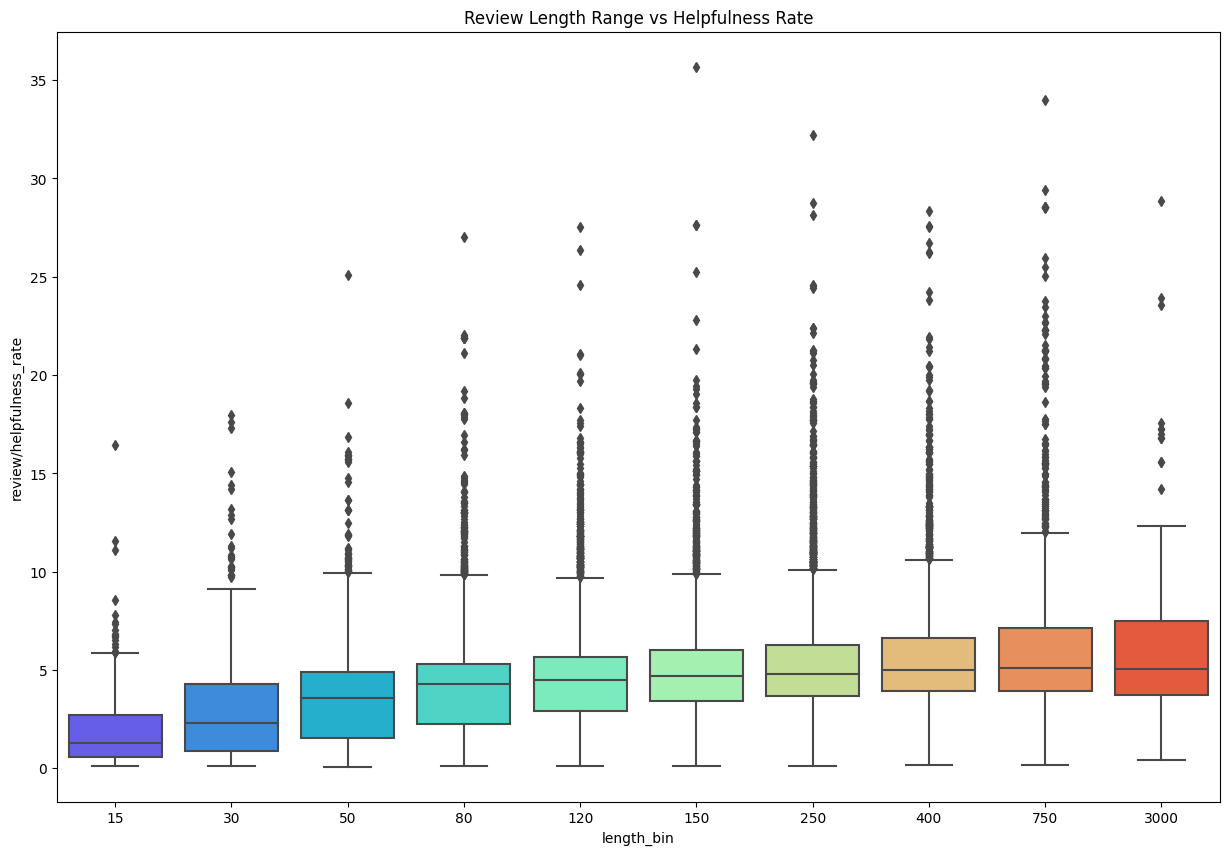
\includegraphics[width=0.49\textwidth]{./figures/h1_boxplot.png}
    \caption{Correlation between review length and helpfulness score for different review length groups}
    \label{fig:h1_boxplot}
\end{figure}

\begin{table}[H]
    \footnotesize
    \centering
    \caption{Correlation Coefficients and P-values for Different Groups}
    \begin{tabular}{|c|c|c|}
    \hline
    Group Number & Correlation Coefficient & P-value \\
    \hline
    400 & 0.2216 & 0.0000 \\
    \hline
    750 & -0.0188 & 0.2585 \\
    \hline
    3000 & -0.1418 & 0.0065 \\
    \hline
    \end{tabular}
    \label{corr_groups}
\end{table}


\subsection*{Hypothesis 2}
This hypothesis investigates whether reviews containing a higher number of positive sentiment words
tend to receive more helpfulness ratings.\\
Before testing this hypothesis, it is necessary to define what is meant by "positive sentiment words".
To do so, a Multinomial Naive Bayes classifier was trained on the dataset,
with adjustments made to consider words with a score greater than 3 as positive reviews and those
with a score less than 3 as negative reviews. Positive sentiment words were identified by calculating
the difference in word weights between the positive and negative classes.
Among these words, those with weights greater than 0 were deemed positive sentiment words.
Only the top 800 words with the highest weights were retained for further analysis.\\
Subsequently, the frequency of these positive sentiment words was computed for each review.
The correlation between the frequency of these words and review helpfulness was then calculated.
Given that the features do not follow a normal distribution, the Spearman correlation coefficient was used.\\
The result yielded a correlation coefficient of 0.318 with a p-value < 0.05, indicating statistical significance in general.
However, the correlation value becomes negative for a number of words higher than 100, as shown in Figure \ref{fig:corr_pos_words}.

\begin{figure}[H]
    \centering
    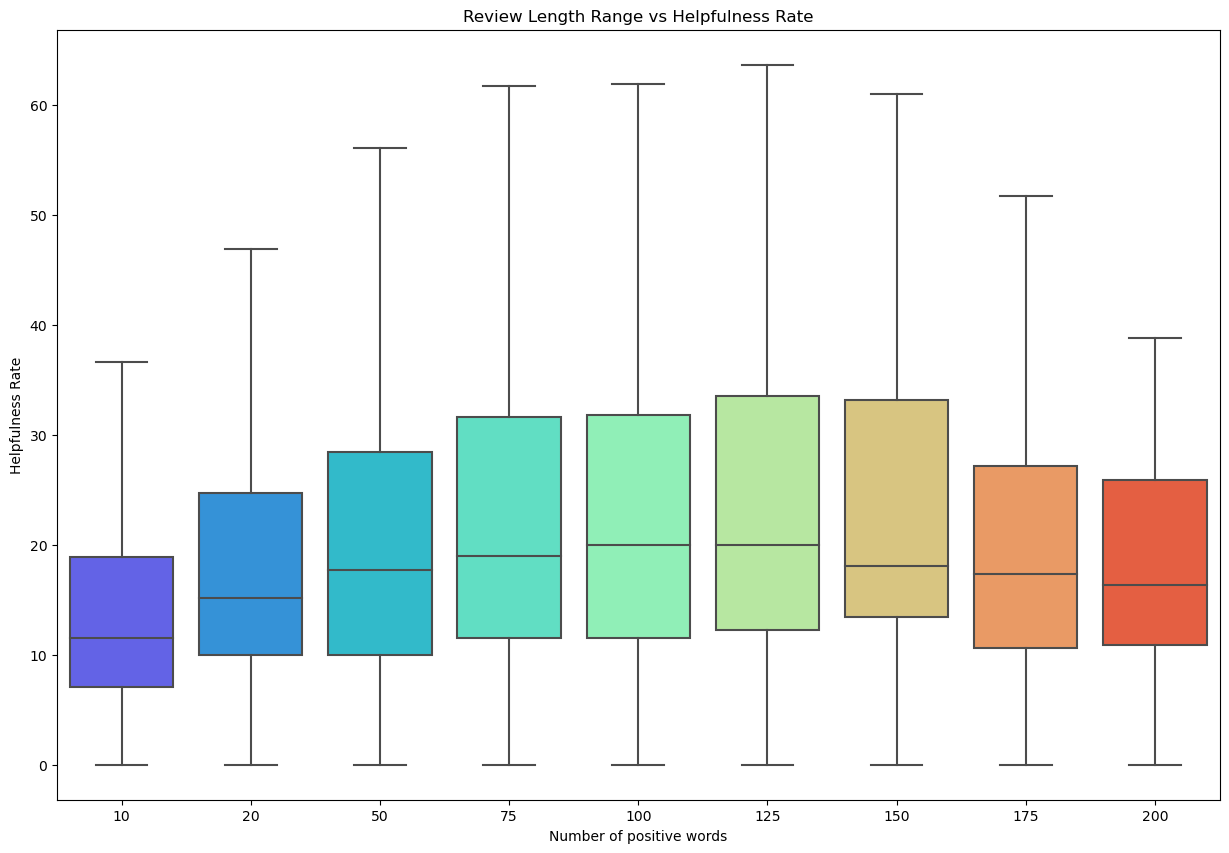
\includegraphics[width=0.4\textwidth]{./figures/h2.png}
    \caption{Correlation between the frequency of positive sentiment words and review helpfulness}
    \label{fig:corr_pos_words}
\end{figure}

\subsection*{Hypothesis 3}

\textbf{H0 (Null Hypothesis):} There is no correlation between the rating of a review and its helpfulness score.\\
\noindent
Similar to the previous hypothesis, we addressed missing values and data transformations directly with a MongoDB query.
With the data prepared for analysis, we conducted an initial examination of the distribution of votes across the four rating
categories. Figure \ref{fig:h3_votes_distribution} reveals a \textbf{positive bias} where individuals tend to vote more for
positive reviews than negative ones. Specifically, a significant portion of votes for rating 5 consists of reviews with a
total vote count equal to 1. This introduces bias into our results because, based on the formula used to compute the
helpfulness score, a small total vote count would lead to a low helpfulness score. To mitigate this, we retained only
reviews with a total vote count greater than 20.

\begin{figure}[H]
    \centering
    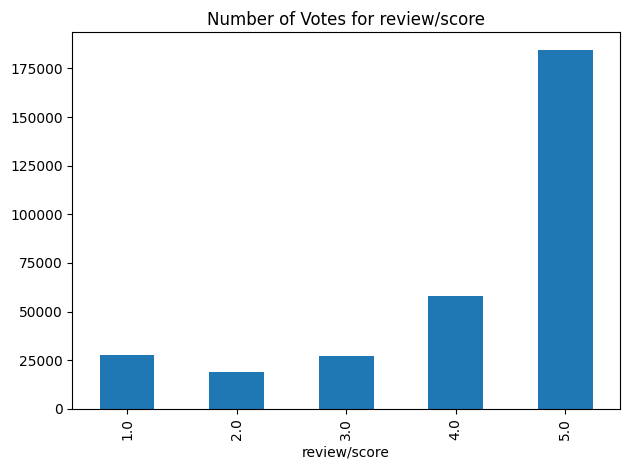
\includegraphics[width=0.4\textwidth]{./figures/h3_votes_distribution.png}
    \caption{Distribution of votes across the four rating categories}
    \label{fig:h3_votes_distribution}
\end{figure}

\noindent
The Spearman correlation coefficient between the two variables is $0.5247$, with a p-value of $0.0$.\\
\textbf{Conclusion:}
The hypothesis is confirmed as there is a positive and statistically significant correlation between the review rating
and helpfulness score. This finding is further supported by the boxplot in Figure \ref{fig:h3_boxplot}.

\begin{figure}[H]
    \centering
    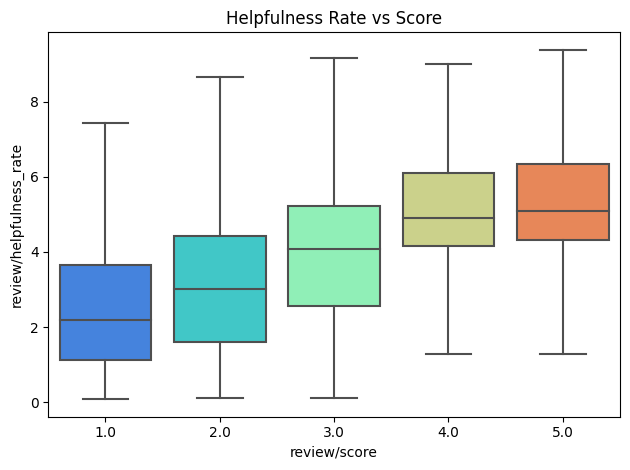
\includegraphics[width=0.3\textwidth]{./figures/h3_boxplot.png}
    \caption{Boxplot illustrating the correlation between review rating and helpfulness score}
    \label{fig:h3_boxplot}
\end{figure}

\subsection*{Hypothesis 4}
Hypothesis 4 explores the impact of individual users' unique personalities, personal preferences,
and the potential for anonymous users to overrate books on rating scores.
We tested this hypothesis by considering the rating score as the primary metric and
any records with missing values were excluded from the analysis.
The hypotheses under examination were as follows:\\
\textbf{H0 (Null Hypothesis):} The rating score is not influenced by the user's profileName.
All rating scores are drawn from the same distribution, implying equal means and variances for each user's rating scores.\\
\textbf{H1 (Alternative Hypothesis):} The rating score is affected by the user,
suggesting that each user's rating scores follow a distinct distribution.\\
For the sake of consistency, users with fewer than 20 reviews were excluded from the analysis,
as a limited number of reviews cannot reliably estimate statistical measures.\\
The statistical test employed was ANOVA, which assesses differences in means between user groups.
The results yielded an F-statistic of 1.5374 and a corresponding P-value of 0.0670.
These results indicate that although there may be some variance in rating scores among different users,
the evidence to reject the null hypothesis (H0) and conclude that user personalities significantly impact
rating scores is not robust.\\
This conclusion is further supported by the accompanying boxplot (Figure \ref{fig:h4}),
which illustrates variations in the distribution of rating scores across users.
\begin{figure}[H]
    \centering
    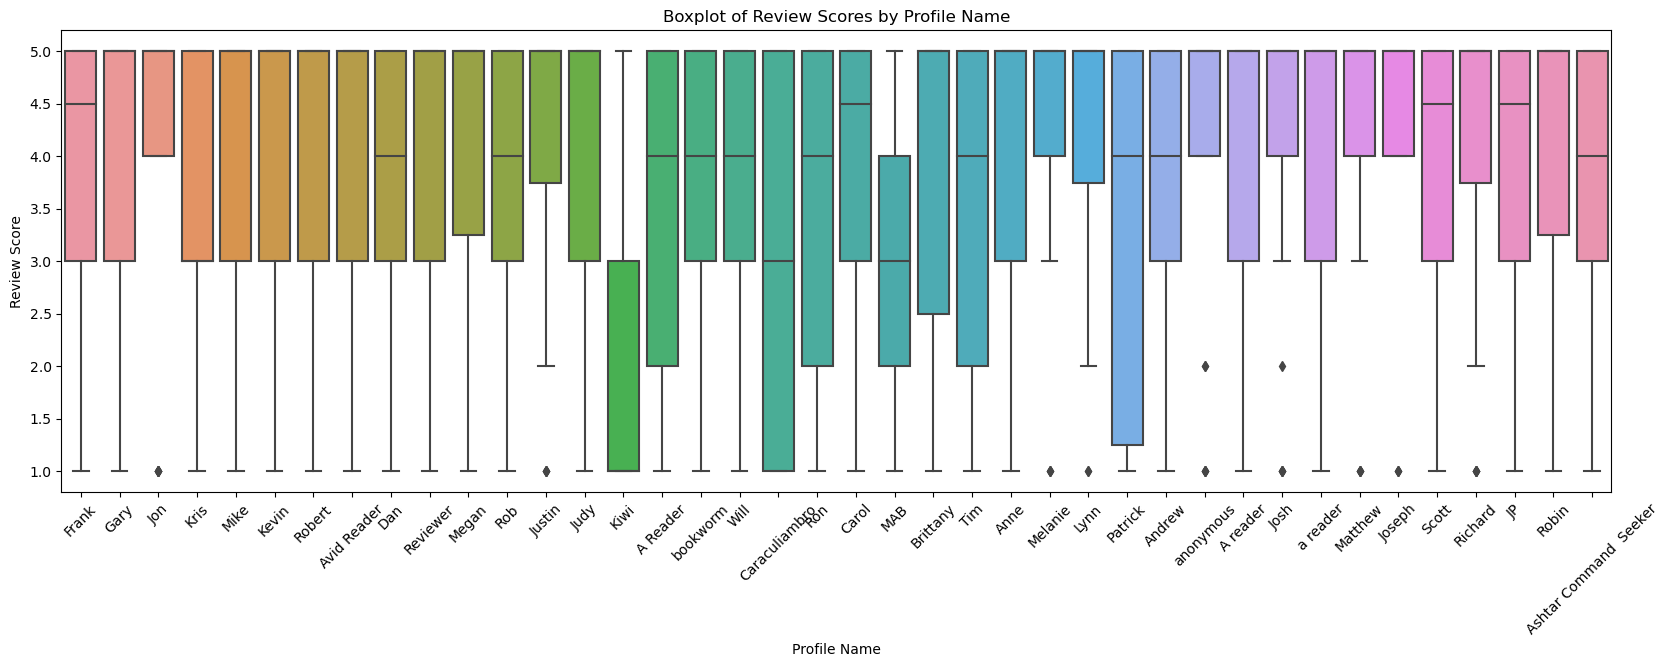
\includegraphics[width=0.5\textwidth]{./figures/h4.1.png}
    \caption{Distribution of rating scores across users}
    \label{fig:h4}
\end{figure}

\subsection*{Hypothesis 5}

Hypothesis 5 examines the influence of book categories on review scores.
To test this hypothesis,we considered the rating score as the metric and removed missing values.
two competing hypotheses were established:\\
\textbf{H0 (Null Hypothesis):} Rating scores are not related to the book categories,
as all rating scores are drawn from the same distribution.\\
\textbf{H1 (Alternative Hypothesis):} Rating scores are affected by the book category,
indicating that the rating scores of each category follow different distributions.\\
As in the previous hypothesis, categories with fewer than 20 reviews were omitted for consistency.
An ANOVA (Analysis of Variance) test was conducted to assess the validity of these hypotheses.
The results of the test revealed an F-statistic of 0.177 and a P-value of 0.999.
A low F-statistic value and a P-value close to 1 suggest that there is not much variation
between the means of different categories.
Therefore, we could not reject the null hypothesis (H0) and concluded that book categories
do not significantly impact rating scores.
This result was further supported by the accompanying boxplot (Figure \ref{fig:h5}),
which showed that the distribution of rating scores was similar across categories.
\begin{figure}[H]
    \centering
    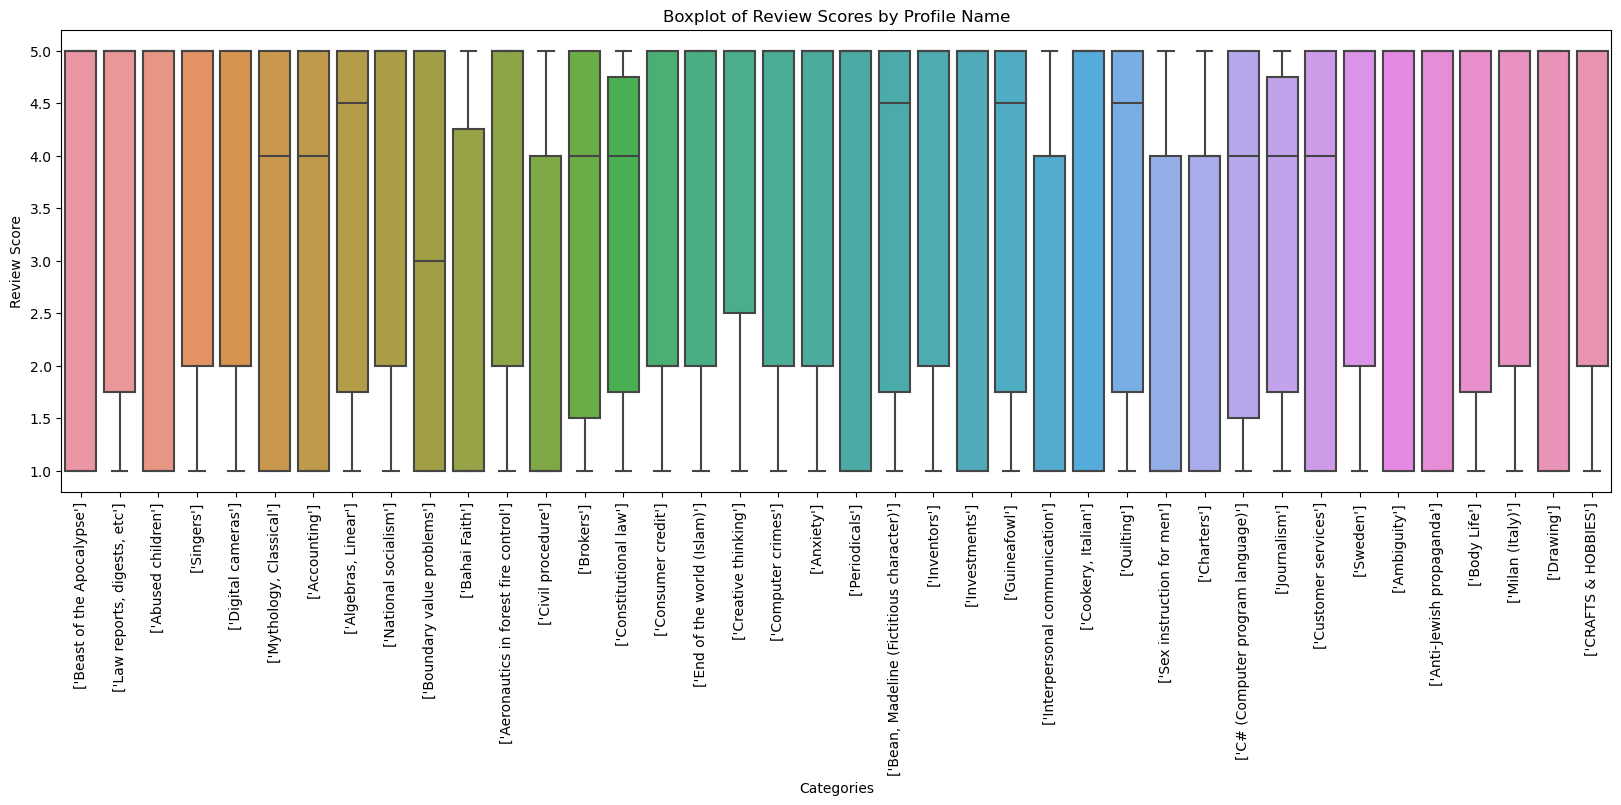
\includegraphics[width=0.5\textwidth]{./figures/h5.png}
    \caption{Distribution of rating scores across categories}
    \label{fig:h5}
\end{figure}

\subsection*{Hypothesis 6}

- The larger the number of books published for a category, the higher the review score.\\ 
- The larger the number of books published by publishers, the higher the review score.\\
\noindent
\textbf{Metric:} Correlation Coefficient.\\
\noindent
\textbf{Missing Values:}
\begin{itemize}
\item \textit{`publisher`:} remove the entire sample
\item \textit{`review/score`:} remove the entire sample
\item \textit{`categories`:} remove the entire sample
\end{itemize}
\noindent
\textbf{Data Transformation:}
\begin{itemize}
    \item \textit{`categories`:} GroupBy categories.
    \item \textit{`publisher`:} GroupBy publisher.
    \item \textit{`review/score`:} Compute the average review/score for each publisher and category.
\end{itemize}\vspace{0.5cm}
\noindent
\textbf{Description and Results}
All the data cleaning and transformation steps were performed using MongoDB with the aggregation pipeline, to have a more efficient and faster computation.\\
Specifically the data cleaning steps were performed using the \textit{\$match} operator, while the data transformation steps were performed using the \textit{\$group} operator with \textit{\$avg} operation.
Finally a \textit{\$project} operator was used to select the fields of interest. To reduce bias, we removed the categories having less than 50 books and the publishers having less than 20 books.\\
The results are shown in Table \ref{tab:h6_correlations}.\\
\textbf{Conclusion:} The hypotheses are falsified since the metrics shows no correlation between the two variables in both cases.

\begin{table}[H]
    \centering
    \caption{Correlation Values and P-values for Categories and Publishers}
    \begin{tabular}{|c|c|c|}
    \hline
    \textbf{Variable} & \textbf{Correlation Value} & \textbf{P-value} \\
    \hline
    Category & -0.0806 & 0.558 \\
    \hline
    Publisher & -0.0673 & 0.151 \\
    \hline
    \end{tabular}
    \label{tab:h6_correlations}
\end{table}

\vspace{0.5cm}
\noindent 
\textbf{Curiosity}
We performed two complex MongoDB queries (reported as example in section 'Code') to answer to two questions:\\
\begin{itemize}
    \item Which are the best publishers? (i.e. capable of getting avg scores above 4.5 in lots of categories)
    \item In which categories are the best publishers focused?
\end{itemize}

The results are reported in Figure \ref{fig:h6_which_best} and Figure \ref{fig:h6_where_best}.

\begin{figure}[H]
    \centering
    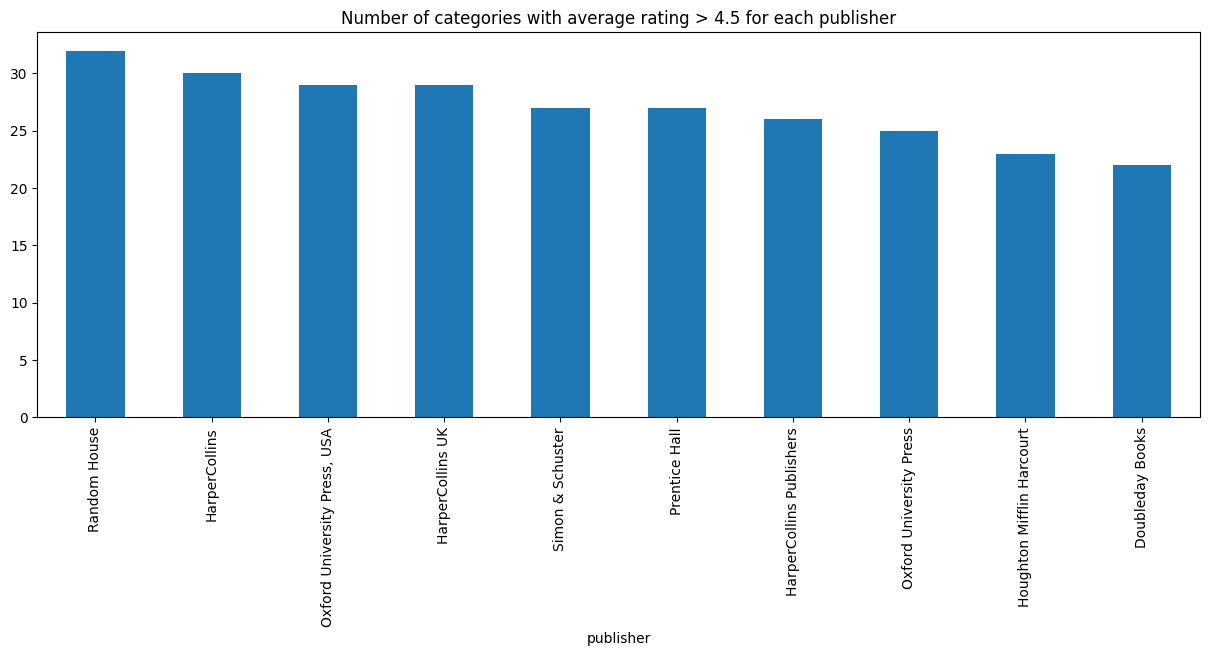
\includegraphics[width=0.5\textwidth]{./figures/h6_which_best.png}
    \caption{Which are the best publishers?}
    \label{fig:h6_which_best}
\end{figure}

\begin{figure}[H]
    \centering
    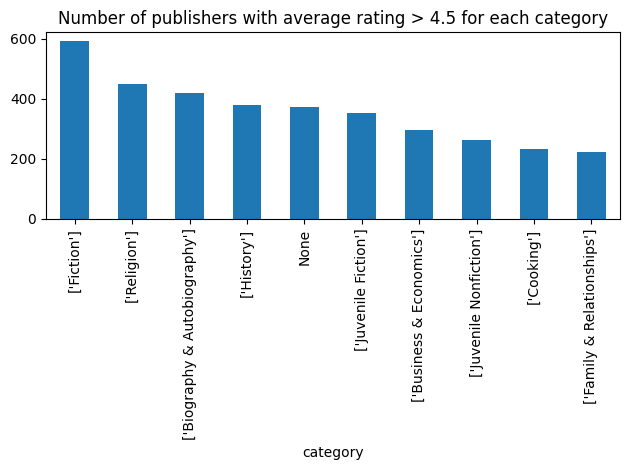
\includegraphics[width=0.5\textwidth]{./figures/h6_where_best.png}
    \caption{In which categories are the best publishers focused?}
    \label{fig:h6_where_best}
\end{figure}
\section{Spark Hypotheses Testing}
To showcase the feasibility of implementing data analysis within a Big Data context, we opted to replicate some hypothesis testing using
Spark, focusing particularly on Hypotheses 1 and 3.

\subsection*{Hypothesis 1}
Addressing this hypothesis involved several key steps:

\begin{itemize}[leftmargin=*, noitemsep]
      \item \textbf{Compute the Helpfulness Score:}
            This was straightforwardly achieved by leveraging the `WithColumn` method of the Spark DataFrame, creating a new column with the updated values.

      \item \textbf{Compute the Text Length:}
            Text length computation was accomplished by utilizing `regexp\_replace` to eliminate punctuation, along with `Tokenizer` and `StopWordsRemover`
            to tokenize the text and remove stop words. Subsequently, a new column containing the text length was generated.

      \item \textbf{Bucketize the Text Length:}
            To address this requirement, we utilized the `Bucketizer` class from Spark MLlib in conjunction with a User Defined Function (UDF) to
            assign appropriate labels to the classes.

      \item \textbf{Compute the Correlation Coefficient:}
            Finally, the correlation coefficient was computed using the `Correlation.corr` method from Spark MLlib, specifically the Spearman correlation
            coefficient. The data was reshaped to conform to the required format using `VectorAssembler`.

\end{itemize}

\subsection*{Hypothesis 2}
To examine this hypothesis, we utilized Spark MLlib's capabilities to build a Naive Bayes model.
This model was trained to identify positive words within the dataset.
Following this, we computed the occurrence of the top 800 most positive words in each review.\\
We then obtained a Spearman correlation coefficient between helpfulness score and number of positive words of 0.318.
\subsection*{Hypothesis 3}
This hypothesis involved computing the helpfulness score and correlation coefficient, both of which were calculated using the same methods
described in the previous hypothesis.

\subsection*{Results}
In all test cases, the results closely mirrored those obtained in the local environment.


\section{Helpfulness Prediction}
Our ambitious goal was that of building a model able to predict the helpfulness of a review, looking only at the text of the review itself.
To create such a model, we needed firstly to convert the text in a machine-readable format, performing a process called \textit{feature extraction}.
Then we tried different models, in order to find the one that best fits our needs eventually selecting the best one.

\subsection{Feature Extraction}
Seen the complexity of the problem we decided to use a \textit{Word Embedding} technique, called \textit{Word2Vec}, that is able to convert a word in a vector of real numbers
while preserving the semantic meaning of the word itself. We used the \textit{Gensim} library to perform this task using the following parameters:
\begin{itemize}[noitemsep, leftmargin=*]
    \item \textbf{Size}: 30
    \item \textbf{Window}: 5
    \item \textbf{Min Count}: 2
    \item \textbf{Workers}: -1
\end{itemize}
As a consequence, each word is represented by a vector of 30 real numbers. The average of the vectors of all the words in a review is the vector representation of the review.

\subsection{Models}
We tried three different models: \textit{Random Forest}, \textit{Support Vector Regressor (RBF kernel)} and \textit{MLP}.
We used the \textit{Scikit-Learn} library to perform the training and the testing of the models. Specifically for this last step
we used the \textit{GridSearchCV} class, that performs a cross-validation on the training set, in order to find the best parameters for the model.
The results are show in Table \ref{tab:model_results} and supported by Figure \ref{fig:model_results}.

\begin{table}[H]
    \footnotesize
    \centering
    \caption{Model Results}
    \label{tab:model_results}
    \begin{tabular}{|c|c|c|c|}
        \hline
        Model & MSE & RMSE & R\textsuperscript{2} \\
        \hline
        RF & 0.0259 & 0.1609 & 0.2532 \\
        SVR & 0.0279 & 0.1670 & 0.1955 \\
        MLP & 0.0282 & 0.1680 & 0.1858 \\
        \hline
    \end{tabular}
\end{table}

\begin{figure}[H]
    \centering
    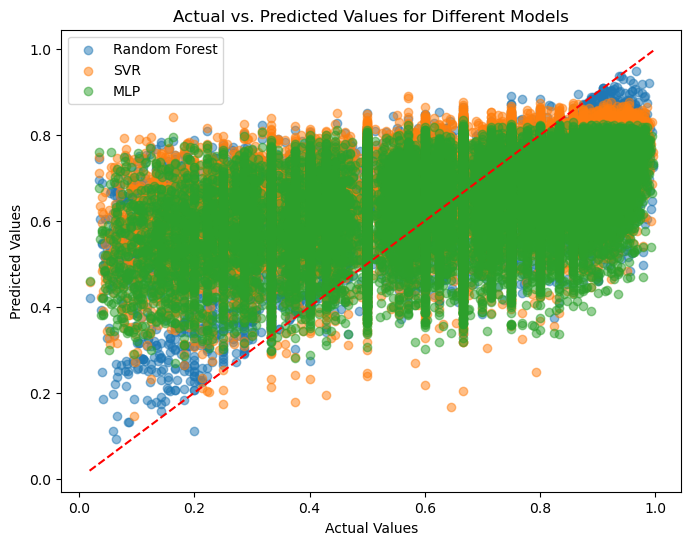
\includegraphics[width=0.48\textwidth]{./figures/model_results.png}
    \caption{Model Results}
    \label{fig:model_results}
\end{figure}

\noindent
As we can see from the graph and the metrics used, the Random Forest model outperforms the other models in terms of Mean Squared Error 
(MSE) and Root Mean Squared Error (RMSE). The Random Forest model achieved the lowest MSE of approximately 0.026 and RMSE of approximately 
0.161, indicating that its predictions are, on average, the closest to the actual values. 
This suggests that Random Forest has the best overall predictive performance among the three models.

\subsection{Results Interpretation}
Figure \ref{fig:model_best_scatter} and Figure \ref{fig:model_best_lines} help us in the results Interpretation.


\begin{figure}[H]
    \centering
    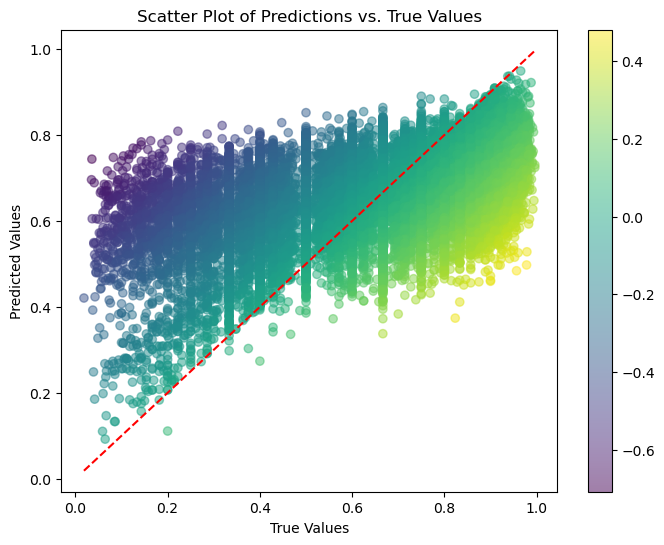
\includegraphics[width=0.48\textwidth]{./figures/model_best_scatter.png}
    \caption{Best Model Errors}
    \label{fig:model_best_scatter}
\end{figure}

\begin{figure}[H]
    \centering
    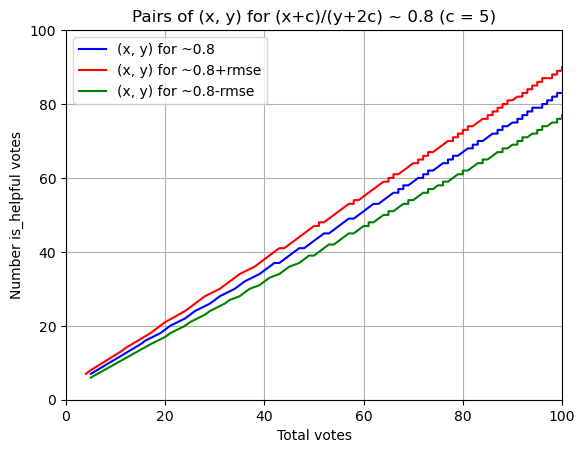
\includegraphics[width=0.48\textwidth]{./figures/model_best_lines.png}
    \caption{Best Model Errors Translation}
    \label{fig:model_best_lines}
\end{figure}





%% Complex MongoDB query to answer: In which categories are the best publishers focused?

\section{Python Script}
\vspace{0.5cm}
This is the script to answer the question: In which categories are the best publishers focused?\\
\lstset{
    language=Python,
    basicstyle=\footnotesize\ttfamily,
    numbers=left,
    numberstyle=\tiny,
    numbersep=5pt
}

\begin{lstlisting}
# Deal with missing values
pipeline_missing = {'$match': {
    'review/score': {'$exists': True, '$ne': 0},
    'publisher': {'$exists': True, '$ne': None},
    'categories': {'$exists': True},
}
}

# Compute average rating for each tuple category, publisher
pipeline_average_rating = {'$group': {
    '_id': {
        'category': '$categories',
        'publisher': '$publisher',
    },
    'avg_score': {'$avg': '$review/score'},
    'count': {'$sum': 1}
}
}

# Show average rating for category for each publisher
pipeline_publisher = {'$group': {
    '_id': '$_id.category',
    'avg_score/publisher': {
        '$push': {
            'publisher': '$_id.publisher',
            'avg_score': '$avg_score',
            'count': '$count'
        }
    }
}
}

# Unwind the list of categories
pipeline_unwind = {'$unwind': '$avg_score/publisher'}

# Remove categories or publisher with less than 'threshold' reviews
threshold = 0
pipeline_remove = {'$match': {
    'avg_score/publisher.count': {'$gte': threshold}
}
}

# Count the number of categories with average rating > 4.5
pipeline_counts = {'$project': {
    'category': '$_id',
    '_id': 0,
    'publisher': '$avg_score/publisher.publisher',
    'count': {
        '$sum': {
            '$cond': {

                'if': {'$gt': ['$avg_score/publisher.avg_score', 4.5]},
                'then': 1,
                'else': 0
            }
        }
    }
}
}

# Sum the results for each publisher. If Total > 10, then the hypothesis is False
pipeline_sum = {'$group': {
    '_id': '$category',
    'total': {'$sum': '$count'}
}
}

pipeline_sort = {'$sort': {
    'total': -1
}
}

results = books.aggregate([pipeline_missing, pipeline_average_rating, pipeline_publisher,
                          pipeline_unwind, pipeline_remove, pipeline_counts,
                          pipeline_sum, pipeline_sort])
\end{lstlisting}




    
\section{Conclusion}

In our exploration of the Amazon Books Review dataset,
we've demonstrated the power of data science to unearth valuable insights.
Our journey began with a dedicated team and ambitious goals, leveraging cutting-edge tools such as Hadoop,
Spark, MongoDB, and Python to tackle big data challenges efficiently.\\
We delved into various hypotheses, examining factors like review length, sentiment,
ratings, and their impact on review helpfulness. Our investigation also ventured into user profiles,
book categories, and their influence on review scores, shedding light on user behavior and preferences.\\
While our journey faced challenges, we persisted. Some hypotheses were confirmed,
while others refined our understanding of book reviews' complexities.\\
In conclusion, our project exemplifies the expanding horizons of data science and the importance of
data-driven decision-making. We remain committed to further exploration and application of these insights,
believing that data science will continue to illuminate our world and shape a data-driven future.
\end{document}
